\documentclass{article}
\usepackage{graphicx} % Required for inserting images

\documentclass[a4paper, 12pt]{article}%тип документа
\usepackage{xcolor}
%отступы
\usepackage[left=2cm,right=2cm,top=2cm,bottom=3cm,bindingoffset=0cm]{geometry}
\usepackage[pdftex]{lscape}
%Русский язык
\usepackage[T2A]{fontenc} %кодировка
\usepackage[utf8]{inputenc} %кодировка исходного кода
\usepackage[english,russian]{babel} %локализация и переносы
\usepackage{multirow}
%Вставка картинок
\usepackage{wrapfig}
\usepackage{graphicx}
\graphicspath{{Images/}}
\DeclareGraphicsExtensions{.pdf,.png,.jpg}

%Математика
\usepackage{amsmath, amsfonts, amssymb, amsthm, mathtools}

%Заголовокhttps://www.overleaf.com/project/6507f5a4176b25bf05722230

\begin{document}

\begin{titlepage}
	\begin{center}
		{\large МОСКОВСКИЙ ФИЗИКО-ТЕХНИЧЕСКИЙ ИНСТИТУТ (НАЦИОНАЛЬНЫЙ ИССЛЕДОВАТЕЛЬСКИЙ УНИВЕРСИТЕТ)}
	\end{center}
	\begin{center}
		{\large Физтех-школа биологической и медицинской физики}
	\end{center}
	
	
	\vspace{4.5cm}
	{\huge
		\begin{center}
			{\bf Отчёт о выполнении лабораторной работы}\\
			Методы статического и динамического рассеяния света для исследования наночастиц и макромолекул в растворах
		\end{center}
	}
	\vspace{3cm}
	\begin{flushright}
		{\LARGE Авторы:\\ Акимов Максим \\ Кондратюк Наталья \\
			\vspace{0.5cm}
			Б06-206}
	\end{flushright}
	\vspace{3cm}
	\begin{center}
		Долгопрудный 
       \\22 сентября 2024 года
	\end{center}
 
\end{titlepage}

\newpage 
\section{Аннотация}

\paragraph*{Цель работы}:
Оценить размер частиц в образцах с помощью методов статического (СРС) и динамического рассеяния света (ДРС), а также познакомиться с соответствующим этим методам техническим оборудованием.
\paragraph*{Задачи}:
\begin{itemize}
        \item ознакомиться с содержанием работы; разобраться с работой спектрометра Photocor Complex и соответствующего ПО (Photocor/DynaLS);
        \item определить размер частиц в образцах с применением программ Photocor и DynaLS; сравнить полученные результаты и погрешности; сделать выводы об этих данных;
        \item провести измерения автокорреляционной функции для разных углов рассеяния; построить индикатрису рассеяния; оценить размер частиц по её виду;
        \item обработать данные, сделать выводы о соответствии результатов теоретически ожидаемым, сделать выводы о работе в целом, сдать и оформить отчёт о выполнении лабораторной работы.
\end{itemize}
\section{Введение}\;
\par \textbf{Рассеяние} – это процесс, в котором молекула или частица заимствует у распространяющейся в среде электромагнитной волны некоторую долю энергии и впоследствии излучает эту энергию в окружающее пространство. Его можно представить в виде схемы из двух частей – возбуждение и переизлучение.
В результате могут происходить изменения характеристик потока излучения: пространственного распределения интенсивности, частотного спектра, поляризации. Помимо переизлучения, часть энергии падающей электромагнитной волны может быть преобразована в другие виды энергии (например, в тепло) – происходит поглощение.

Различают два типа рассеяния.
Неупругое рассеяние, приводящее к появлению в рассеянном свете линий $\omega0 \pm \Omega$, смещённых по частоте относительно возбуждающего излучения $\omega$. \textbf{Упругое} – рассеяние света, сопровождающееся перераспределением энергии
между излучением и веществом, происходящее без существенного изменения частоты. 
Диапазоны:\newline
1. \textit{Рэлея} ($d < \frac{\lambda}{15}$ ) - все элементарные диполи рассеивающей частицы излучают в одной фазе;\newline
2. \textit{Ми} ($\frac{\lambda}{15} \leq d \leq \lambda $) - переизлучение первичной
волны элементарными диполями;\newline
3. \textit{Фраунгофера} (d $> \lambda$) - преимущественно происходит процесс дифракции.
Методы ДРС и СРС основываются на предположении об упругом рассеянии света.
В теории Рэлея предполагается, что электромагнитное излучение, проходя через среду, взаимодействует с ней, индуцируя появление диполей, являющихся источником вторичного излучения, распространяющегося во всех направлениях, кроме своей оси, с той же длиной волны, что и падающий свет.

Теория Ми применяется, когда характерные размеры рассеивающих центров соизмеримы со световой длиной волны. В этом случае интенсивность рассеяния зависит как от концентрации раствора, так и от угла рассеяния.

Если же размер частицы превышает длину волны падающего света, то происходит преимущественно процесс дифракции(Фраунгофера). Информация о размере частицы заключается в величине малого угла дифракционного расхождения.
\subsection{ Метод статического рассеяния света}\;
\par В экспериментах по СРС регистрируется усреднённая по времени интенсивность рассеянного образцом света. Анализ угловых зависимостей и зависимостей от концентрации
интенсивности рассеянного света позволяет получить информацию о размерах и некоторых (влияющих на масштаб флуктуаций оптических свойств) термодинамических свойствах рассеивающих центров.
Во многих практических приложениях используются макромолекулы и частицы с размерами в диапазоне от нанометров до микрон. Под размером в методах СРС подразумевается радиус инерции - Rg - величина, характеризующая распределение элементарных
излучателей в частице или макромолекуле:
\[ R^2_{g} = \frac{ \sum \limits_{i} m_{i} r^2_{i}}{\sum\limits_{i} m_{i}} \]


Суммарная интенсивность рассеянного света I зависит от длины световой волны $\lambda$
(в вакууме), интенсивности падающего света $I_{0}$, рассеивающего объёма $\omega$, расстояния
от рассеивающего объёма до приёмника x, поляризуемости частицы $\alpha$, концентрации
рассеивающих частиц $n_{0}$ и угла рассеяния $\theta$:
\[I =\frac{16\pi^4}{\lambda^4x^2 }\alpha^2n_{0}\Omega I_{0} P(\Theta)\]

где P($\Theta$) - коэффициент формы.
Поляризуемость излучающей частицы, пропорциональна объёму частицы , если образующие частицу элементарные диполи излучают в одной фазе (это условие выполняется
для достаточно малых частиц) $\alpha \sim d^3$
. Из приведённой выше формулы следует, что
интенсивность пропорциональна шестой степени размера частицы: $ I \sim \alpha^2 \sim d^6$
.

\textbf{Индикатриса рассеяния} - диаграмма направленности излучения, графически отображающая зависимость интенсивности рассеянного света от угла рассеяния.
Вид угловой зависимости рассеяния $P(\Theta)$ определяется размерами и формой рассеивающих частиц.

В зависимости от размеров рассеивающих частиц, показателей преломления и направления наблюдения интерференция волн может усиливать или ослаблять интенсивность рассеянного света. В случае рэлеевского рассеяния все диполи внутри частицы излучают в одной фазе, поэтому интенсивность рассеянного излучения для всех $\theta$ совпадает с
максимально возможной (при заданном количестве элементарных диполей).
Для более крупных частиц удобно провести нормировку на максимальную интенсивность рассеянного излучения, рассчитываемую по теории Рэлея. Эффекты интерференции описываются коэффициентом формы $P(\Theta)$, введенным ранее:

\[I(\Theta) = P(\Theta) · I(0) \]

Коэффициент формы всегда меньше или равен 1.
\subsection{Метод динамического рассеяния света}\;
\par Методы динамического светорассеяния
позволяют определить время жизни флуктуации. Одной из разновидностей ДРС является метод фотонной корреляционной спектроскопии.

В данном методе изучается корреляция (во времени) количества фотонов,
рассеянных образцом в заданном направлении. В качестве источника излучения
используется лазер. Электромагнитные волны, рассеянные соседними частицами, интерферируют друг с другом. Возникающие при этом временные флуктуации интенсивности рассеянного света формируют на фотодетекторе сигнал I(t), характерные времена изменения которого обусловлены броуновским движением рассеивающих частиц. 


Прибор, называемым коррелятором, который строит автокорреляционную функцию сигнала. Автокорреляционная функция показывает корреляцию значений сигнала (в
данном случае – интенсивности рассеянного света) измеренных через промежу-
ток времени $\tau$.
\begin{equation}
    g_2(\tau) = \; <I(t)I(t+\tau)>
\end{equation}

АКФ электрического поля, называемая корреляционной функцией первого
порядка (в отличие от корреляционной функции второго порядка для
интенсивности поля), вводится аналогично:
\begin{equation}
    g_1(\tau) = \;<E^*(t)E(t+\tau)>
\end{equation}

Электрическое поле как падающей, так и рассеянной волн линейно поляризовано, поэтому рассмотрим только z-компоненту поля. Электрическое поле световой волны, рассеянной на флуктуациях показателя преломления среды в направлении вектора $k'$, можно представить в виде $E(t) = \delta E(t)*e^{-i\omega_0 t)}$.
Медленно меняющаяся со временем амплитуда поля $ \delta E(t)$ пропорциональна флуктуации концентрации рассеивающих частиц с волновым вектором q, ответственным за рассеяние согласно условию Брэгга:
 \begin{equation}
     \delta C_{\Vec{q}}(\Vec{r}, t) = \delta A \cdot sin(\Vec{q} \cdot \Vec{r})
 \end{equation}
 \begin{equation}
     \delta E(t)  = A \cdot \delta C_{\Vec{q}}(\Vec{r}, t).
 \end{equation}

Здесь подразумевается, что флуктуации представлены в виде пространственного Фурье-разложения. В соответствии с гипотезой Онзагера, релаксация микроскопических флуктуаций концентрации к равновесному состоянию может быть описана уравнением диффузии:
\begin{equation}
    \frac{\partial C}{\partial t} = D \Delta C.
\end{equation}
Согласно этому уравнению флуктуации концентрации экспоненциально затухают с течением времени.
Причём величина, обратная времени жизни такой флуктуации, равна:
\begin{equation}
    1/t_{c}= D \cdot q^2.
\end{equation}

В этом случае автокорреляционная функция электрического поля рассеянного излучения затухает также по экспоненциальному закону с тем же характерным временем.
Таким образом, по результатам аппроксимации автокорреляционной функции интенсивности рассеянного света можно определить коэффициент диффузии частиц. Далее, исходя из него, размер частиц может быть найден из формулы Стокса–Эйнштейна:

\begin{equation}
    D = \frac{k_{b} T}{6\pi R \eta}.
\end{equation}

\section{Описание установки}
В данной работе используется Photocor Complex для измерения параметров диспергированных в жидкости наноразмерных частиц. 

На жестком основании смонтированы прецизионный гониометр и оптическая скамья, на которой размещены диодный лазер Photocor-DL ($\lambda_{0}=$
658,6 нм) и фокусирующий узел. Термостат и адаптер кювет установлены на
гониометре коаксиально с его осью. На поворотной консоли гониометра располагается фотоприемный блок, в состав которого входит приемная оптическая
система со сменной диафрагмой выбора апертуры, малошумящий фотоумножитель, работающий в режиме счета фотонов, быстрый усилитель-дискриминатор
со сквозным по постоянному току трактом и специальный высоковольтный источник питания ФЭУ без паразитных корреляций. 


\begin{figure}[!htb] 
        \minipage{0.5\textwidth}
            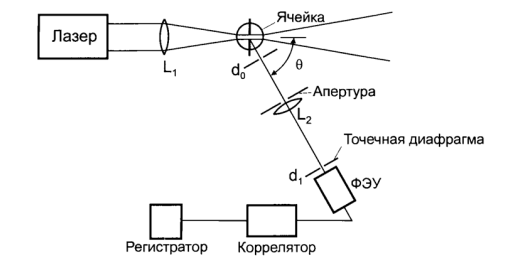
\includegraphics[width=1.3\linewidth]{Images/ДВА.png}
                 \caption{Принципиальная схема прибора.}
        \endminipage\hfill
        \minipage{0.5\textwidth}
             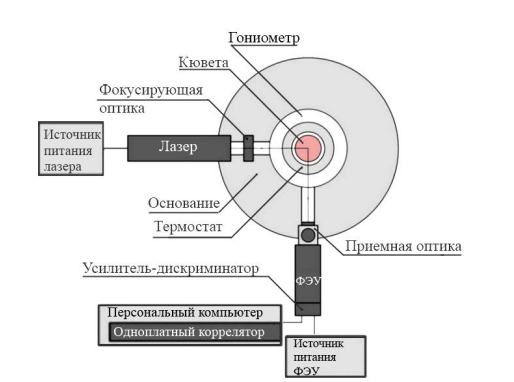
\includegraphics[width=0.88\linewidth]{Images/ОДИН.png}
                 \caption{Схема прибора Photocor Complex.}
        \endminipage
\end{figure}

\section{Результаты и обсуждение}\;
\par В работе метод динамического рассеяния света применялся к двум коллоидным растворам: раствор серы в ацетоне и золь золота. В обоих случаях измерения проходили по следующей схеме:
\begin{itemize}
    \item Кювета с исследуемым раствором помещалась в соответствующее отделение прибора Photocor Complex;
    \item На кювету падает свет от лазера, который рассеивается на коллоидных частицах в растворе;
    \item Рассеянный свет под некоторым фиксированным углом детектируется приёмной оптикой и через ФЭУ попадает в регистратор, а затем в компьютер (угол пробегает значения от $20^{\circ}$ до $140^{\circ}$ с шагом в $10^{\circ}$);
    \item С помощью программ Photocor и DynaLS на выходе получаем следующие данные: интенсивность рассеяния (+STD) и время корреляции (+STD);
\end{itemize}
\par Дальнейшая обработка данных сводится к построению зависимости из формулы (6), определению коэффициента диффузии и размера частиц по формуле (7). При этом модуль вектора рассеяния высчитывается по следующей формуле:
$$q = \frac{4\pi n}{\lambda_0}\sin{\frac{\theta}{2}}$$
\par Для определения характера рассеяния частиц и определения примерного соотношения длины волны $\lambda$ и размера частиц $d$ строится индикатриса рассеяния - зависимость $\frac{I_{\theta}\sin{\theta}}{I_{90}}$ от $\theta$ в декартовых и полярных координатах.
\subsection{Коллоидный раствор золотых частиц}\;
\par Коллоидный раствор золотых частиц приготавливался в дистиллированной воде. Таким образом, показатель преломления раствора очень близок к таковому для дистиллированной воды: $n \approx 1,333$. Соберём полученные экспериментальные данные и вычисления на их основе в Таблицу \ref{Таблица 1}.
\begin{table}[h!]
\centering
\caption{Данные ДРС для коллоидного раствора золотых частиц}
\label{Таблица 1}
\begin{tabular}{|l|l|l|l|l|l|}
\hline
$\theta$, $^{\circ}$ & $q, \cdot 10^7 \text{м}^{-1}$  & $t_{c}$, мс & $STD$ & $I, \cdot 10^3$ усл. ед. & $STD, \cdot 10^3$ \\ \hline
20 & 0,44 &  4,379 &  0,982 &  835 &  40 \\ \hline
30 & 0,66 &  1,767 &  0,603 &  630 &  20 \\ \hline
40 & 0,87 &  1,123 &  0,272 &  495 &  15 \\ \hline
50 & 1,07 &  0,713 &  0,23 &  418 &  6 \\ \hline
60 & 1,27 &  0,453 &  0,179 &  366 &  6 \\ \hline
70 & 1,46 &  0,335 &  0,101 &  356 &  8 \\ \hline
80 & 1,63 &  0,288 &  0,085 &  338 &  6 \\ \hline
90 & 1,80 &  0,213 &  0,027 &  328 &  8 \\ \hline
100 & 1,95 &  0,183 &  0,052 &  330 &  5 \\ \hline
110 & 2,08 &  0,183 &  0,051 &  351 &  5 \\ \hline
120 & 2,20 &  0,157 &  0,037 &  370 &  6 \\ \hline
130 & 2,31 &  0,135 &  0,039 &  402 &  10 \\ \hline
140 & 2,39 &  0,713 &  0,144 &  468 &  6 \\ \hline
\end{tabular}
\end{table}
По этим данным построим зависимость $\frac{1}{t_c}(q^2)$, изображённую на Рис. \ref{fig: Сера 1} 


\newpage
\begin{figure}[h!]
\centering
    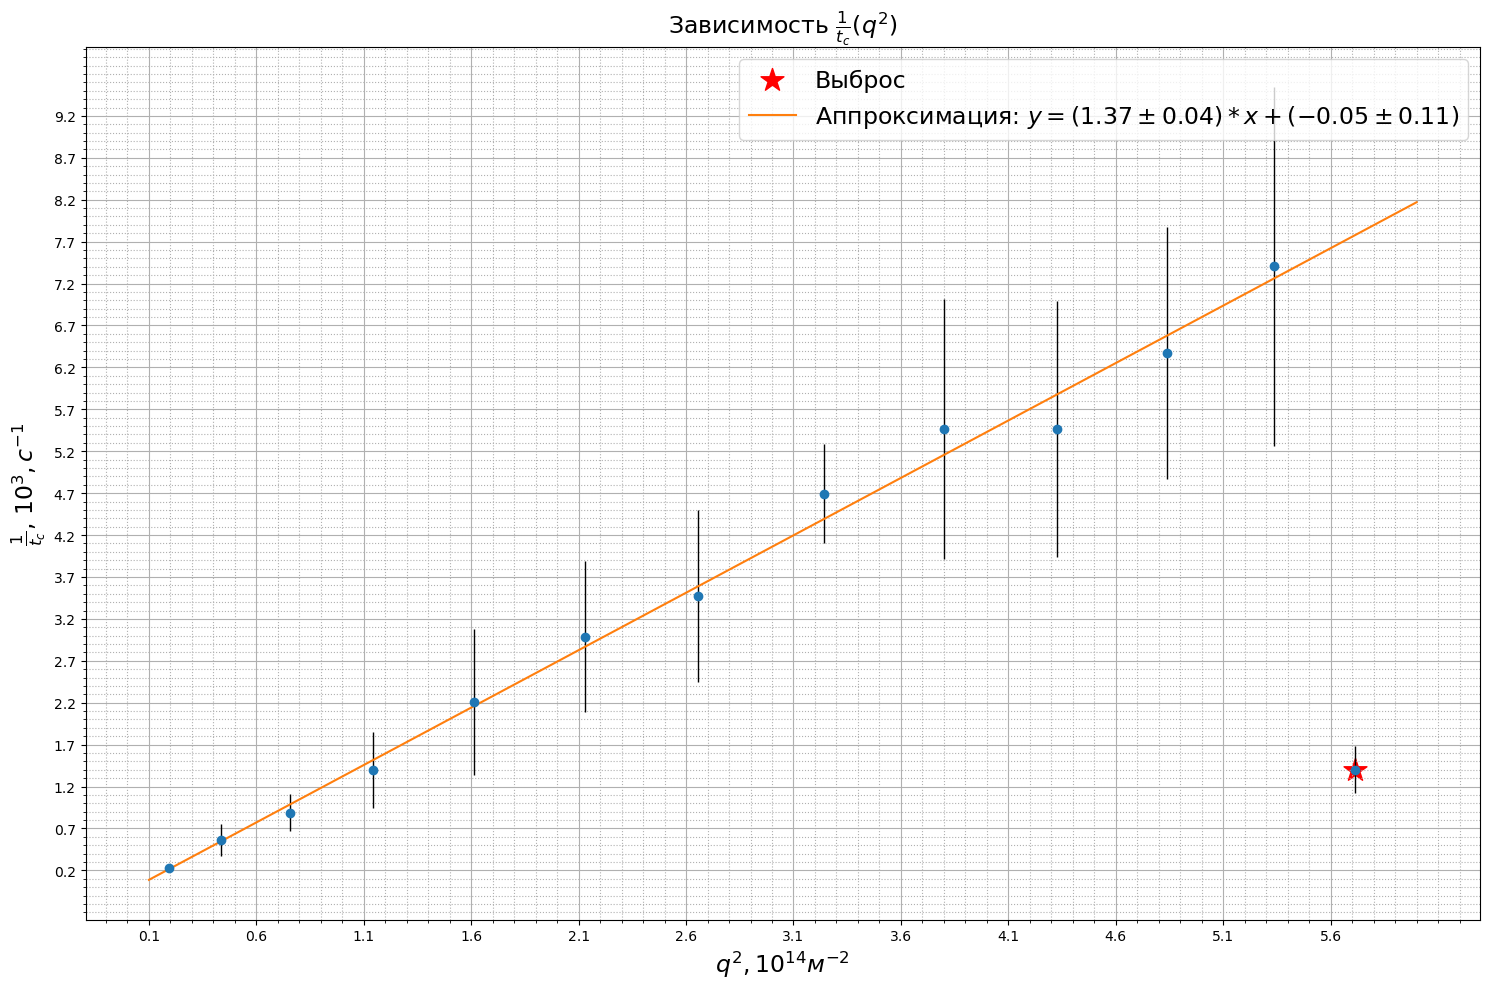
\includegraphics[width=0.8\linewidth]{Images/Сера 1.png}
    \caption{Зависимость $\frac{1}{t_c}(q^2)$ для ДРС золя золота.}
    \label{fig: Сера 1}
\end{figure}
По МНК и с учётом погрешностью МНК и погрешностью анализируемых данных получаем следующее значение коэффициента диффузии:
$$D = (1,4 \pm 0,5) \cdot 10^{-11} \; \frac{\text{м}^2}{\text{с}}$$


Оценим размер частиц по формуле (7) ($T = 295\; K, \eta(20^{\circ}C) = 0,9579 \cdot 10^{-3} \text{Па} \cdot \text{с}$):
$$R = (16 \pm 6)\;\text{нм}, \; d = (32 \pm 12) \;\text{нм}$$


Учитывая длину волны лазера, можем отметить, что в данном случае применима теория рассеяния Рэлея: $d < \frac{\lambda}{15}$.

Чтобы окончательно в этом убедиться, построим индикатрисы рассеяния в декартовых и полярных координатах (Рис. \ref{Сера 2} и Рис. \ref{Сера 3})
\begin{figure}[!htb] 
        \centering
        \minipage{0.45\textwidth}
        \centering
            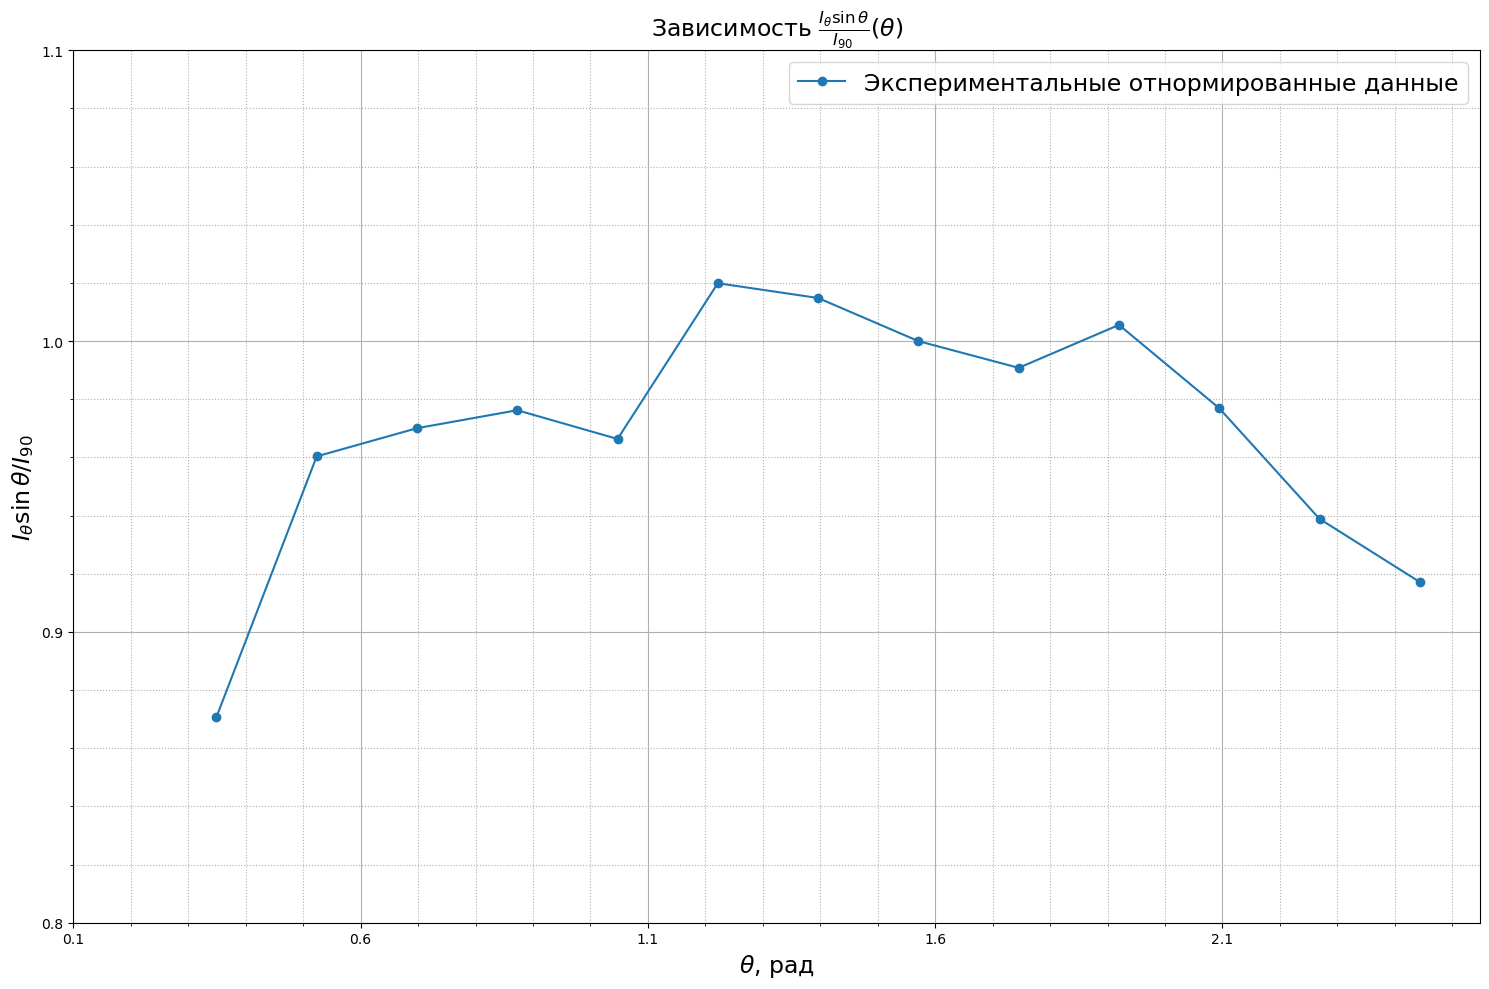
\includegraphics[width=1\linewidth]{Images/Сера 3.png}
                 \caption{Индикатриса рассеяния в декартовых координатах.}
                 \label{Сера 2}
        \endminipage\hfill
        \minipage{0.45\textwidth}
        \centering
             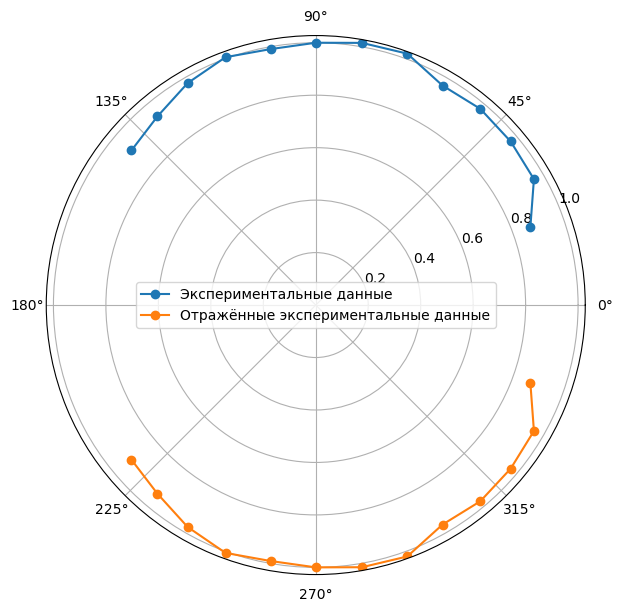
\includegraphics[width=0.69\linewidth]{Images/Сера 2.png}
                 \caption{Индикатриса рассеяния в полярных координатах.}
                 \label{Сера 3}
        \endminipage
\end{figure}

Оценивая индикатрису в декартовых координатах, можно отметить, что нормированное значение интенсивности хоть и меняется, но укладывается в 10\% погрешность. Также заметно, что в полярных координатах, в целом, индикатрисы выглядит симметрично. Следовательно, наши предположения о рассеянии Рэлея были верны и оценка для размеров частиц золота применима ($d < \frac{\lambda}{15} = 43,9 \;\text{нм}$)
\subsection{Коллоидный раствор серы в ацетоне}\
\par Аналогичную обработку проведём для коллоидного раствора серы.
\begin{table}[h!]
\centering
\caption{Данные ДРС для коллоидного раствора серы}
\label{Таблица 1}
\begin{tabular}{|l|l|l|l|l|l|}
\hline
$\theta$, $^{\circ}$ & $q, \cdot 10^7 \text{м}^{-1}$  & $t_{c}$, мс & $STD$ & $I, \cdot 10^3$ усл. ед. & $STD, \cdot 10^3$ \\ \hline
20  & 0,44 & 42,34        & 4,95  & 1250           & 150                \\ \hline
30  & 0,66 & 26,9         & 6,62  & 860            & 80                 \\ \hline
40  & 0,87 & 17,09        & 5,356 & 630            & 50                 \\ \hline
50  & 1,07 & 8,02         & 2,91  & 480            & 40                 \\ \hline
60  & 1,27 & 5,094        & 1,703 & 400            & 25                 \\ \hline
70  & 1,46 & 4,379        & 1,577 & 345            & 30                 \\ \hline
80  & 1,63 & 3,236        & 0,846 & 295            & 15                 \\ \hline
90  & 1,8  & 1,767        & 0,546 & 280            & 10                 \\ \hline
100 & 1,95 & 2,056        & 0,793 & 260            & 10                 \\ \hline
110 & 2,08 & 2,056        & 0,531 & 250            & 10                 \\ \hline
120 & 2,2  & 2,056        & 0,499 & 244            & 10                 \\ \hline
130 & 2,31 & 1,519        & 0,412 & 260            & 12                 \\ \hline
\end{tabular}
\end{table}
\par По этим данным построим зависимость $\frac{1}{t_c}(q^2)$, изображённую на Рис. \ref{fig: Настоящая сера 1}

\begin{figure}[h!]
\centering
    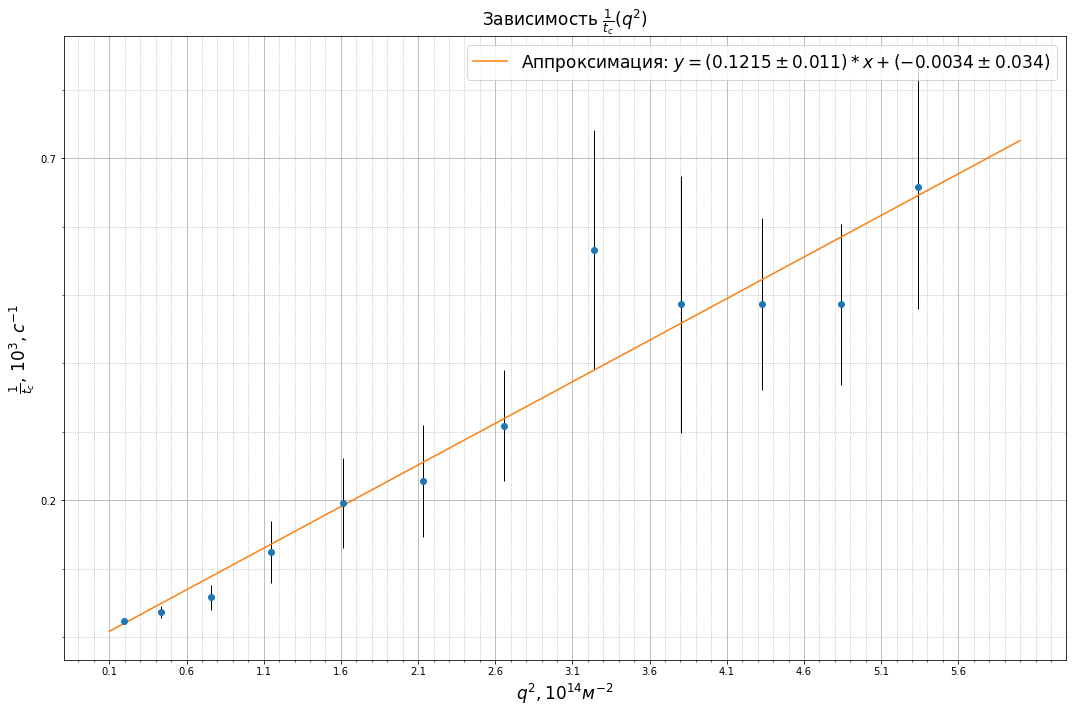
\includegraphics[width=0.8\linewidth]{Images/Сера.png}
    \caption{Зависимость $\frac{1}{t_c}(q^2)$ для ДРС коллоидного раствора серы.}
    \label{fig: Настоящая сера 1}
\end{figure}

\par По МНК и с учётом погрешностью МНК и погрешностью анализируемых данных получаем следующее значение коэффициента диффузии:
$$D = (0,12 \pm 0,05) \cdot 10^{-11} \; \frac{\text{м}^2}{\text{с}}$$


\par Оценим размер частиц по формуле (7):
$$R = (184 \pm 76) \;\text{нм}, \; d = (368 \pm 152) \;\text{нм}$$
\par Учитывая длину волны лазера, можем отметить, что в данном случае применима теория рассеяния Ми: $d > \frac{\lambda}{15}$. А также, рассмотрим индикатрисы рассеяния в декартовых и полярных координатах (Рис. 7 и 8).
\begin{figure}[!htb] 
        \centering
        \minipage{0.45\textwidth}
        \centering
            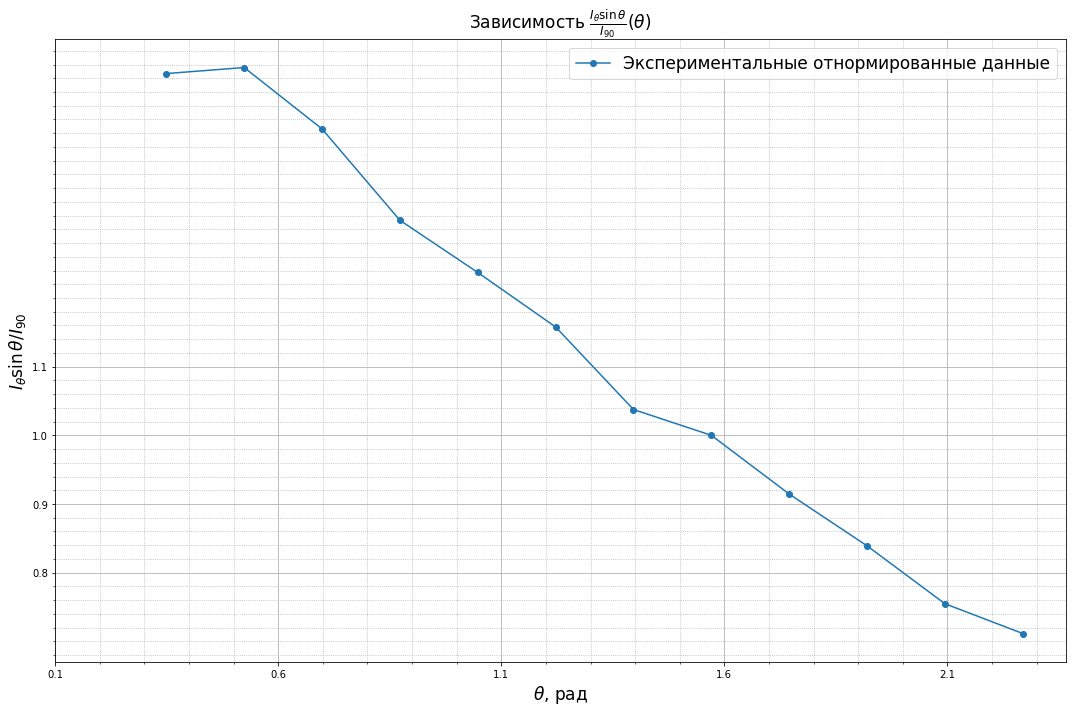
\includegraphics[width=1\linewidth]{Images/декарт.png}
                 \caption{Индикатриса рассеяния для серы в декартовых координатах.}
        \endminipage\hfill
        \minipage{0.45\textwidth}
        \centering
             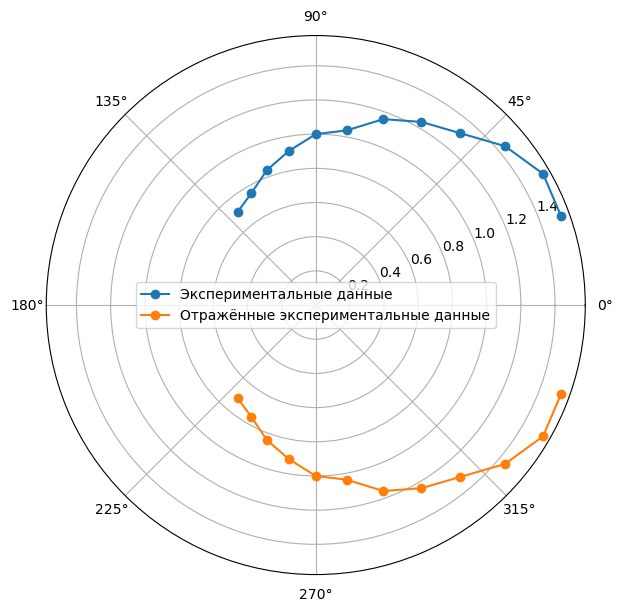
\includegraphics[width=0.69\linewidth]{Images/индикатрисса.jpg}
                 \caption{Индикатриса рассеяния для серы в полярных координатах.}
        \endminipage
\end{figure}
\subsection{Автокорреляционная функция}
 Для угла 90$^{\circ}$ для образцов серы и золота проведем анализ автокорелляционной функции, имеющей следующий вид:
\begin{equation}
   G(t) = \langle I(t)I(t-\tau) \rangle = \lim_{\Delta t\rightarrow\infty}\frac{1}{\Delta t}\int_{0}^{\Delta t} I(t)I(t-\tau)\,dt
\end{equation}
Заметим, что частицы золота меньше, т.к. экспонента начинает убывать на меньших каналах соответствующих меньшим временам. Каналы и времена сконвертированы в соответствии с руководством пользователя ($\tau = 2^{n/8} \cdot 10^{-8}$).

\begin{figure}[!htb] 
        \centering
        \minipage{0.5\textwidth}
        \centering
            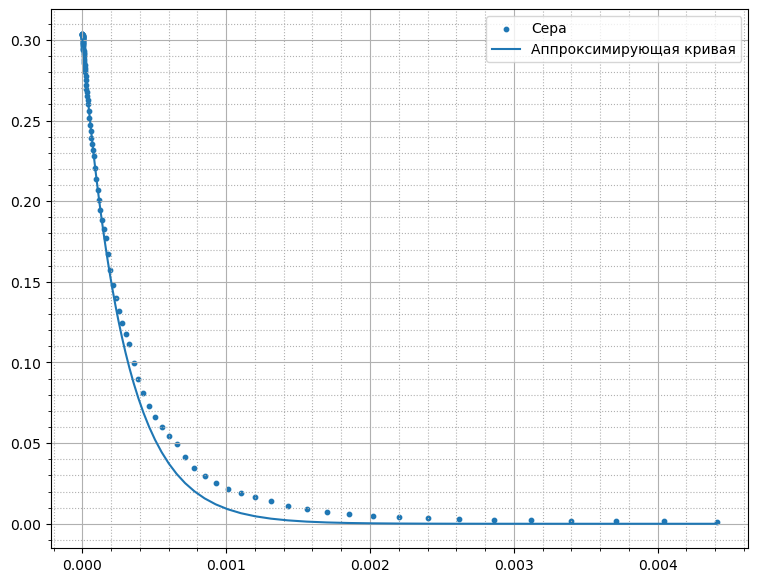
\includegraphics[width=0.7\linewidth]{Images/afk Сера.png}
                 \caption{АФК коллоида серы}
        \endminipage\hfill
        \minipage{0.5\textwidth}
        \centering
             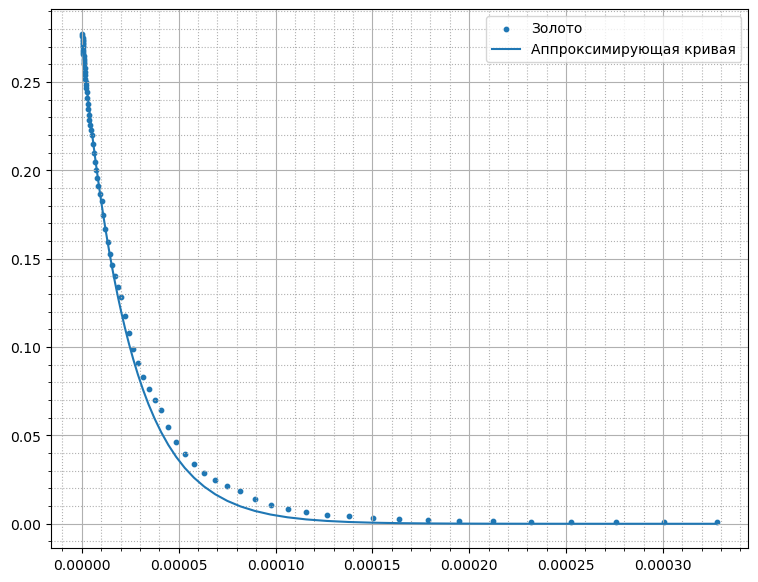
\includegraphics[width=0.7\linewidth]{Images/afk Золото.png}
                 \caption{АФК коллоида золота}
        \endminipage
\end{figure}
\newpage
\begin{figure}[h!]
\centering
    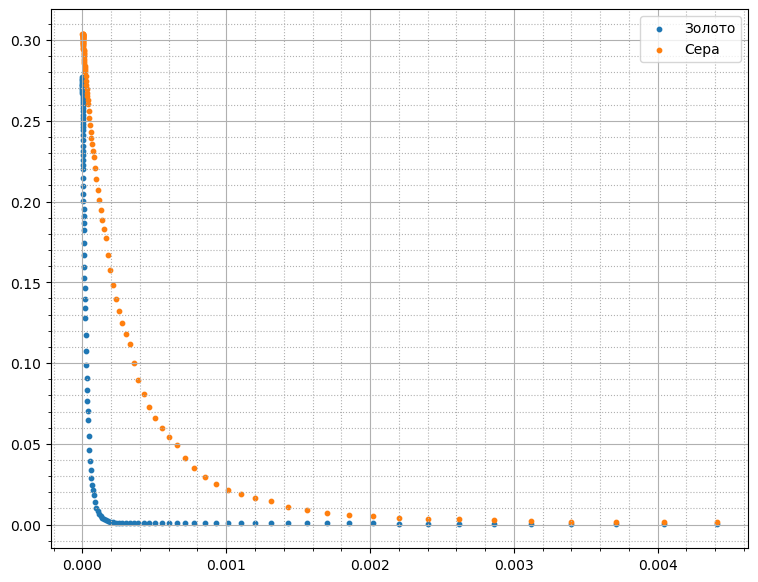
\includegraphics[width=0.8\linewidth]{Images/АФК.png}
    \caption{Сравнение АФК коллоида серы и АФК коллоида золота.}
\end{figure}

На основе аппроксимаций АФК рассчитаем $t_c$: 
$$Au: \frac{1}{t_c} = 4.06 \cdot 10^{4}$$
$$S: \frac{1}{t_c} = 3.27 \cdot 10^{3}$$

Из $t_c$ нетрудно получить значение коэффициента диффузии и радиус частиц:
$$Au: D = 1,25 \cdot 10^{-10} \; \frac{\text{м}^2}{\text{с}};\; R = 7,9 \;\text{нм}$$
$$S:  D = 1,01 \cdot 10^{-11} \; \frac{\text{м}^2}{\text{с}};\; R = 97,4 \;\text{нм} $$

\subsection{Выводы}
\begin{itemize}
    \item В ходе работы с помощью метода динамического светового рассеяния были установлены размеры частиц золота и серы в коллоидных растворах:
    $$d_{\text{золота}} = (32 \pm 12) \;\text{нм}$$
    $$d_{\text{серы}} = (368 \pm 152) \;\text{нм}$$
    \item Исходя из диаметров молекул предполагаем, что для маленьких частиц золота выполняется теория Рэлея, а для более крупных частиц серы - теория Ми.
    \item Индикатрисы рассеяния для обоих коллоидных растворов согласуются с представлением о размерах частиц, полученным динамическим методом. Частицы серы крупнее, из-за этого преобладает рассеяние вперёд (интенсивность рассеяния выше в направлении излучателя).
    $$d_{\text{золота}} \in [10, 20] \;\text{нм}$$
    $$d_{\text{серы}} \in [150, 200] \;\text{нм}$$
    \item По результатам обработки с помощью экспоненциальной аппроксимации 4 порядка автокорреляционной функции были получены значения
    $$d_{\text{золота}} = 15,8\;\text{нм}$$
    $$d_{\text{серы}} = 194,8 \;\text{нм}$$
\end{itemize}

\end{document}
